\chapter{Diseño Y Estructura}

En este capítulo se describe el diseño final del funcionamiento de la aplicación y se explican los elementos que han influido en las decisiones.


\section{Descripción general}
La solución propuesta, se compone de dos componentes diferenciados , por un lado una aplicación Android y por otro lado un servicio web.

El servicio se comporta como una interface entre la aplicación Android y la plataforma ERP\textsuperscript{\textit{[\ref{glo:erp}]}} que dispone el cliente. A través de la base de datos del ERP el servicio recupera los datos necesarios para proveer a la aplicación Android y también inserta los prepedidos realizados por la misma.

Una de las principales características de la aplicación Android, es que tiene que disponer de los datos necesarios para operar, aunque no dispongamos de conexión en este momento. Para ello dispone de una opción de sincronización de sus datos almacenados con los datos actualizados por la empresa. Para optimizar su rendimiento intentado realizar el menor numero de conexiones, se puede configurar el nº de registros por conexión queremos recuperar.

A efectos de estructurar los datos durante las comunicaciones, la opción elegida es el estándar JSON, que sera explicado mas adelante. 

En la siguiente figura podemos ver un esquema, mostramos de una manera esquemática como es la comunicación entre las partes.

\begin{figure}[H]
	\centering
	\fcolorbox{black}{white}{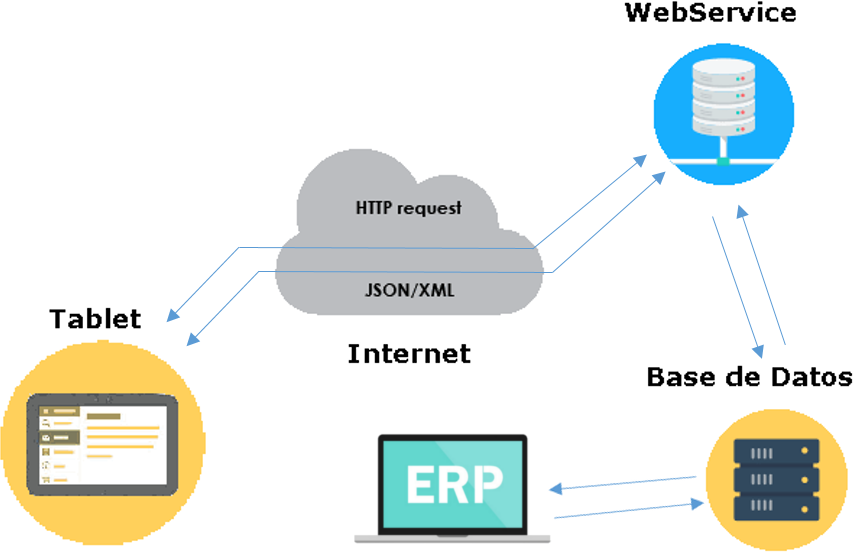
\includegraphics[width=0.9\linewidth]{figuras/esquema}}
	\caption{Esquema principal del proyecto}
	\label{fig:esquema}
\end{figure}


\section{Servicio web}
\subsection{Descripción general}
Antes de abordar la descripción general vamos a definir el termino faceta para su comprensión posterior.
\begin{shaded}
	\begin{flushleft}
	Una faceta, es un aspecto configurable para ejecutar una determinada tarea, cumplir determinados requisitos o tener determinadas características. Por ejemplo, la faceta \textbf{EAR} configura un proyecto para que funcione como una aplicación de empresa añadiendo un descriptor de despliegue y configurando la \textbf{classpath} del proyecto. 
	\end{flushleft}			
\end{shaded}
Dicho esto, dentro del entorno elegido \textit{(Eclipse Oxygen)} hemos elegido un tipo de proyecto \textbf{Dynamic Web Project} que implementa de serie una colección de facetas que serán de ayuda a la hora de desarrollar el servicio web.

\begin{itemize}
	
	\item \emph{\textbf{Dynamic Web Module 3.0: }} Añade soporte para la generación de contenido web dinámico en el API de Servilleta Java.
	\item \emph{\textbf{Java 1.8: }} Añade soporte para la escritura de aplicaciones en  Java.
	\item \emph{\textbf{JavaScript 1.0: }} Permite el desarrollo de Suscriptor utilizando múltiples archivos de origen en una ruta de inclusión configurable.
	\item \emph{\textbf{JAX-RS (REST Web Services) 2.0: }} Permite que el proyecto se implemente con las capacidades de \textbf{JAX-RS}.
\end{itemize}
\subsection{Metodología empleada}
Como hemos comentado en apartados anteriores la elección del tipo de especificación ha sido \textbf{REST}. Al usar esta especificación debemos cumplir con una estructura definida, extbf{JAX-RS}.
\subsubsection{JAX-RS}
Es una \textbf{API} del lenguaje de programación Java que proporciona soporte en la creación de servicios web de acuerdo con el estilo arquitectónico \textbf{REST \textit{(Representational State Transfer)}}. \textbf{JAX-RS} usa anotaciones, introducidas en Java SE 5, para simplificar el desarrollo y despliegue de los clientes y puntos finales de los servicios web.\cite{jaxrs}

\subsection{Diseño e implementación}
Una vez configurado el tipo de proyecto en Eclipse, elegimos \textbf{MAVEN} \textsuperscript{\textit{[\ref{glo:maven}]}} como su constructor de proyectos.

Durante el desarrollo usaremos anotaciones \textsuperscript{\textit{[\ref{glo:anota}]}}, que nos proporciona por defecto \textbf{JAX-RS}, esto nos permite relacionar las URIS del servicio web con el código fuente de una manera mas intuitiva. 

En el ejemplo siguiente mostramos el código fuente correspondiente a la URI : \textit{http://[servidor:puerto]/[servicio]/sincroniza/totales }.\\


\begin{lstlisting}[style=JAVA]
	@Path(value = "/sincroniza")
	public class InTrazaWS {
		
		@GET
		@Path("totales")
		@Produces(MediaType.APPLICATION_JSON)
		public Totales consultaTotalesBD() { 
			return JDBCQuery.getRegistrosTotales(); }	
		.......		
	}
\end{lstlisting}

Vamos a disponer de varias etiquetas de anotación que nos van a proveer de los métodos necesarios para la comunicación con el servicio.

\begin{lstlisting}

@GET - doGet del Servlet
@POST - doPost del Servlet
@Path("prepedido") - path final de la uri
@Consumes(MediaType.APPLICATION\_JSON) consulta por JSON
@Produces(MediaType.APPLICATION\_JSON) escritura por JSON 

\end{lstlisting}

Debemos de definir las rutas para recuperar/insertar los diferentes conjuntos de datos con los que trabajará la aplicación Android. A continuación mostramos un listado de los mismos:\\

\begin{itemize}	
	\item \textbf{totales: } consultaTotalesBD 
	\item \textbf{artículos: } consultaArticulosBD 
	\item \textbf{clientes: } consultaClientesBD 
	\item \textbf{ruteros total fraccionados: } getRuterosTotalFraccionados 
	\item \textbf{rutero tarifa cliente: } consultaTarifaClienteRuteroBD 
	\item \textbf{rutero peso total anio: } consultaPesoTotalAnioRuteroBD 
	\item \textbf{rutero datos: } consultaDatosParaRuteroBD
	\item \textbf{pre-pedido: } enviaPrepedidoBD	\\	
\end{itemize}
 
Cada elemento del listado corresponde a un objeto o conjunto de objetos que se ha procesado de una cadena de caracteres estructurada bajo la especificación \textbf{JSON}. 

Tanto para insertar como para obtener los elementos, se realizaran a través de los métodos del listado, que implementan toda la lógica de operación de la base de datos del cliente, a través del conector java correspondiente. En este caso \textbf{Postgre SQL}.

\subsection{Diagramas}

En la siguiente figura vemos el diagrama \textbf{UML} con las clases principales del servicio web, los accesos a través de intrazaWs y su relación esquemática.\\

\begin{figure}[H]
	\centering
	\fcolorbox{black}{white}{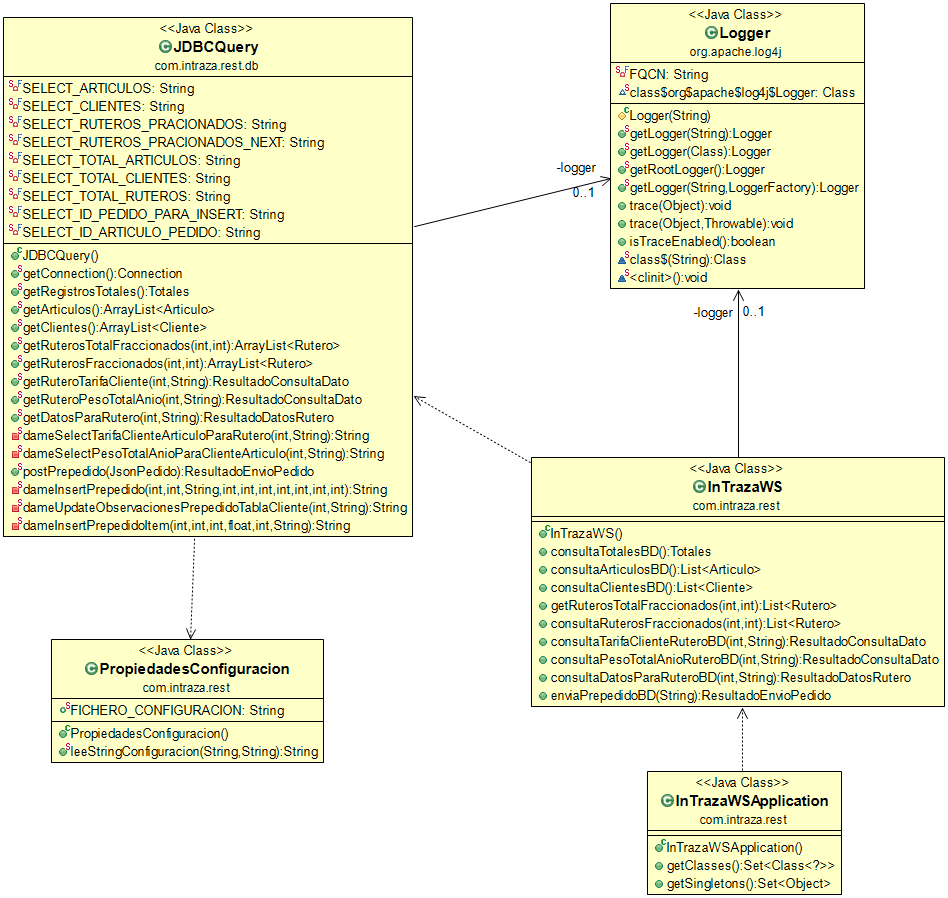
\includegraphics[width=0.58\linewidth]{figuras/dia-web-ser-gen}}
	\caption{Esquema principal del proyecto}
	\label{fig:dia-web-ser-gen}
\end{figure}

\pagebreak

En la siguiente figura vemos el diagrama \textbf{UML} con las relaciones de los objetos transformables a partir de la cadena recibida con la especificación \textbf{JSON}.\\

\begin{figure}[H]
	\centering
	\fcolorbox{black}{white}{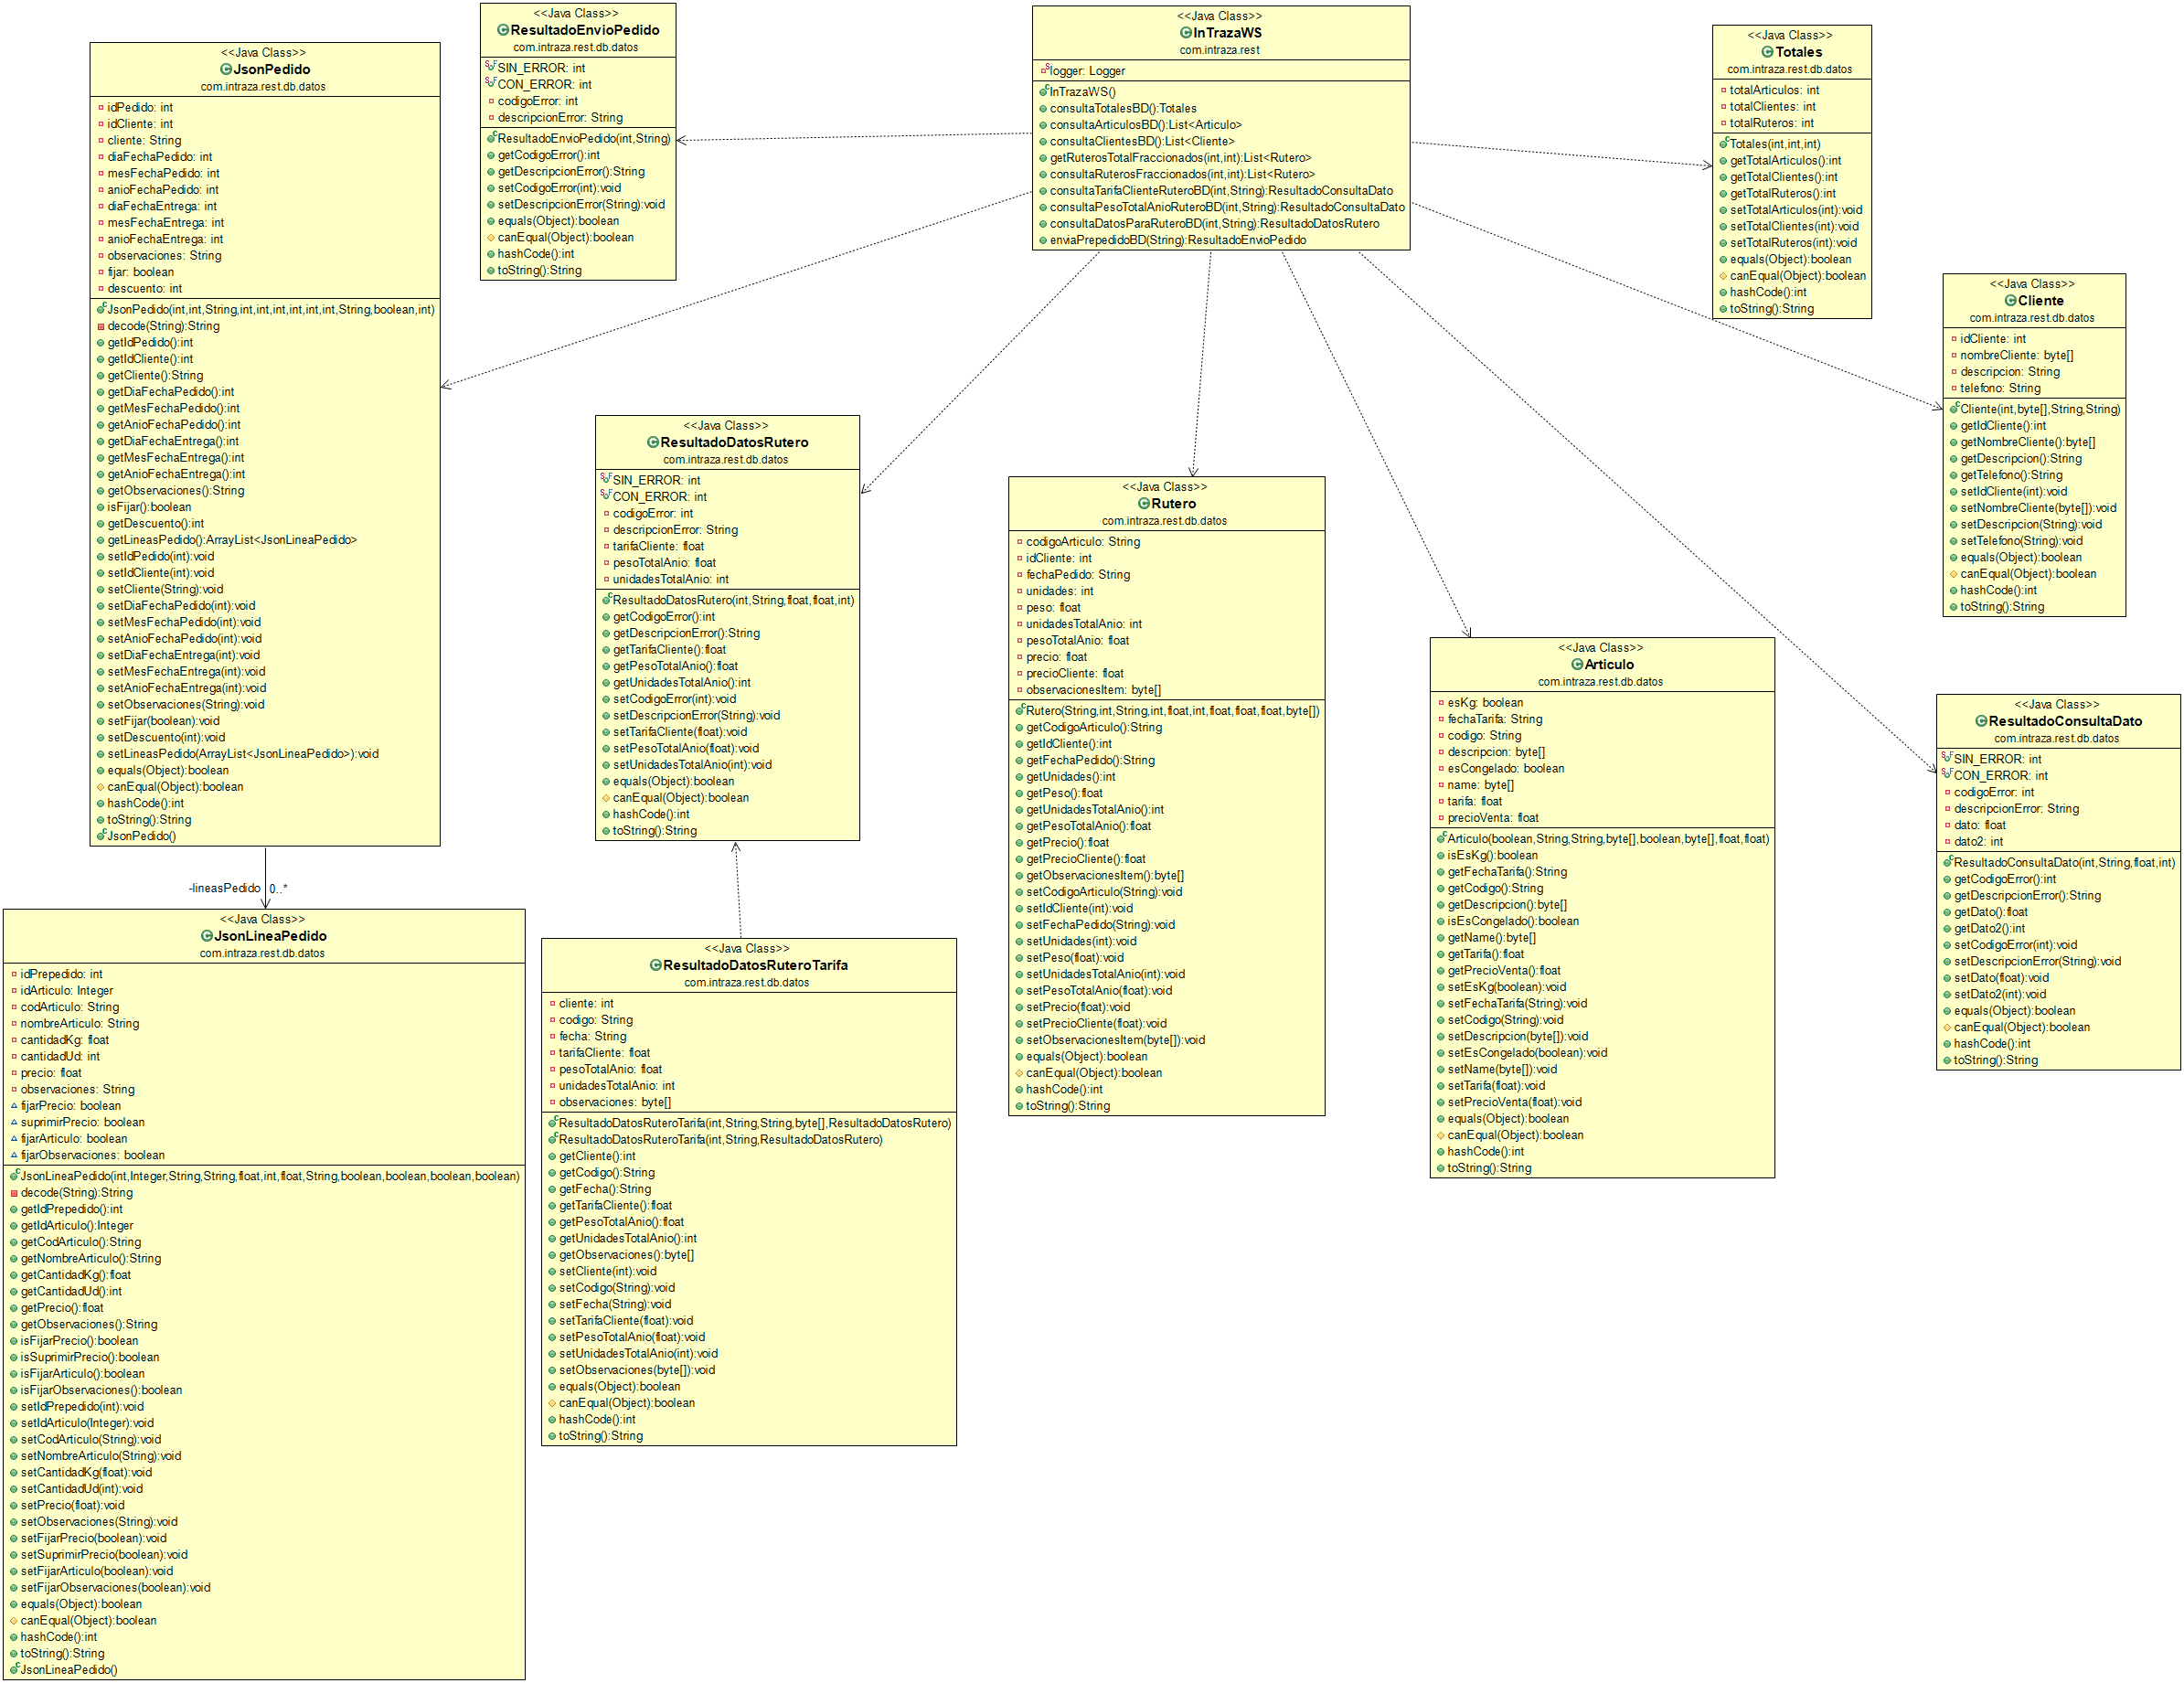
\includegraphics[width=0.9\linewidth,angle=270]{figuras/dia-web-ser}}
	\caption{Relaciones de datos}
	\label{fig:dia-web-ser}
\end{figure}

\pagebreak

En la siguiente figura vemos el diagrama \textbf{UML} con la relación de la clase que gestiona la comunicación con la Base de datos y las clases objeto del servicio.\\

\begin{figure}[H]
	\centering
	\fcolorbox{black}{white}{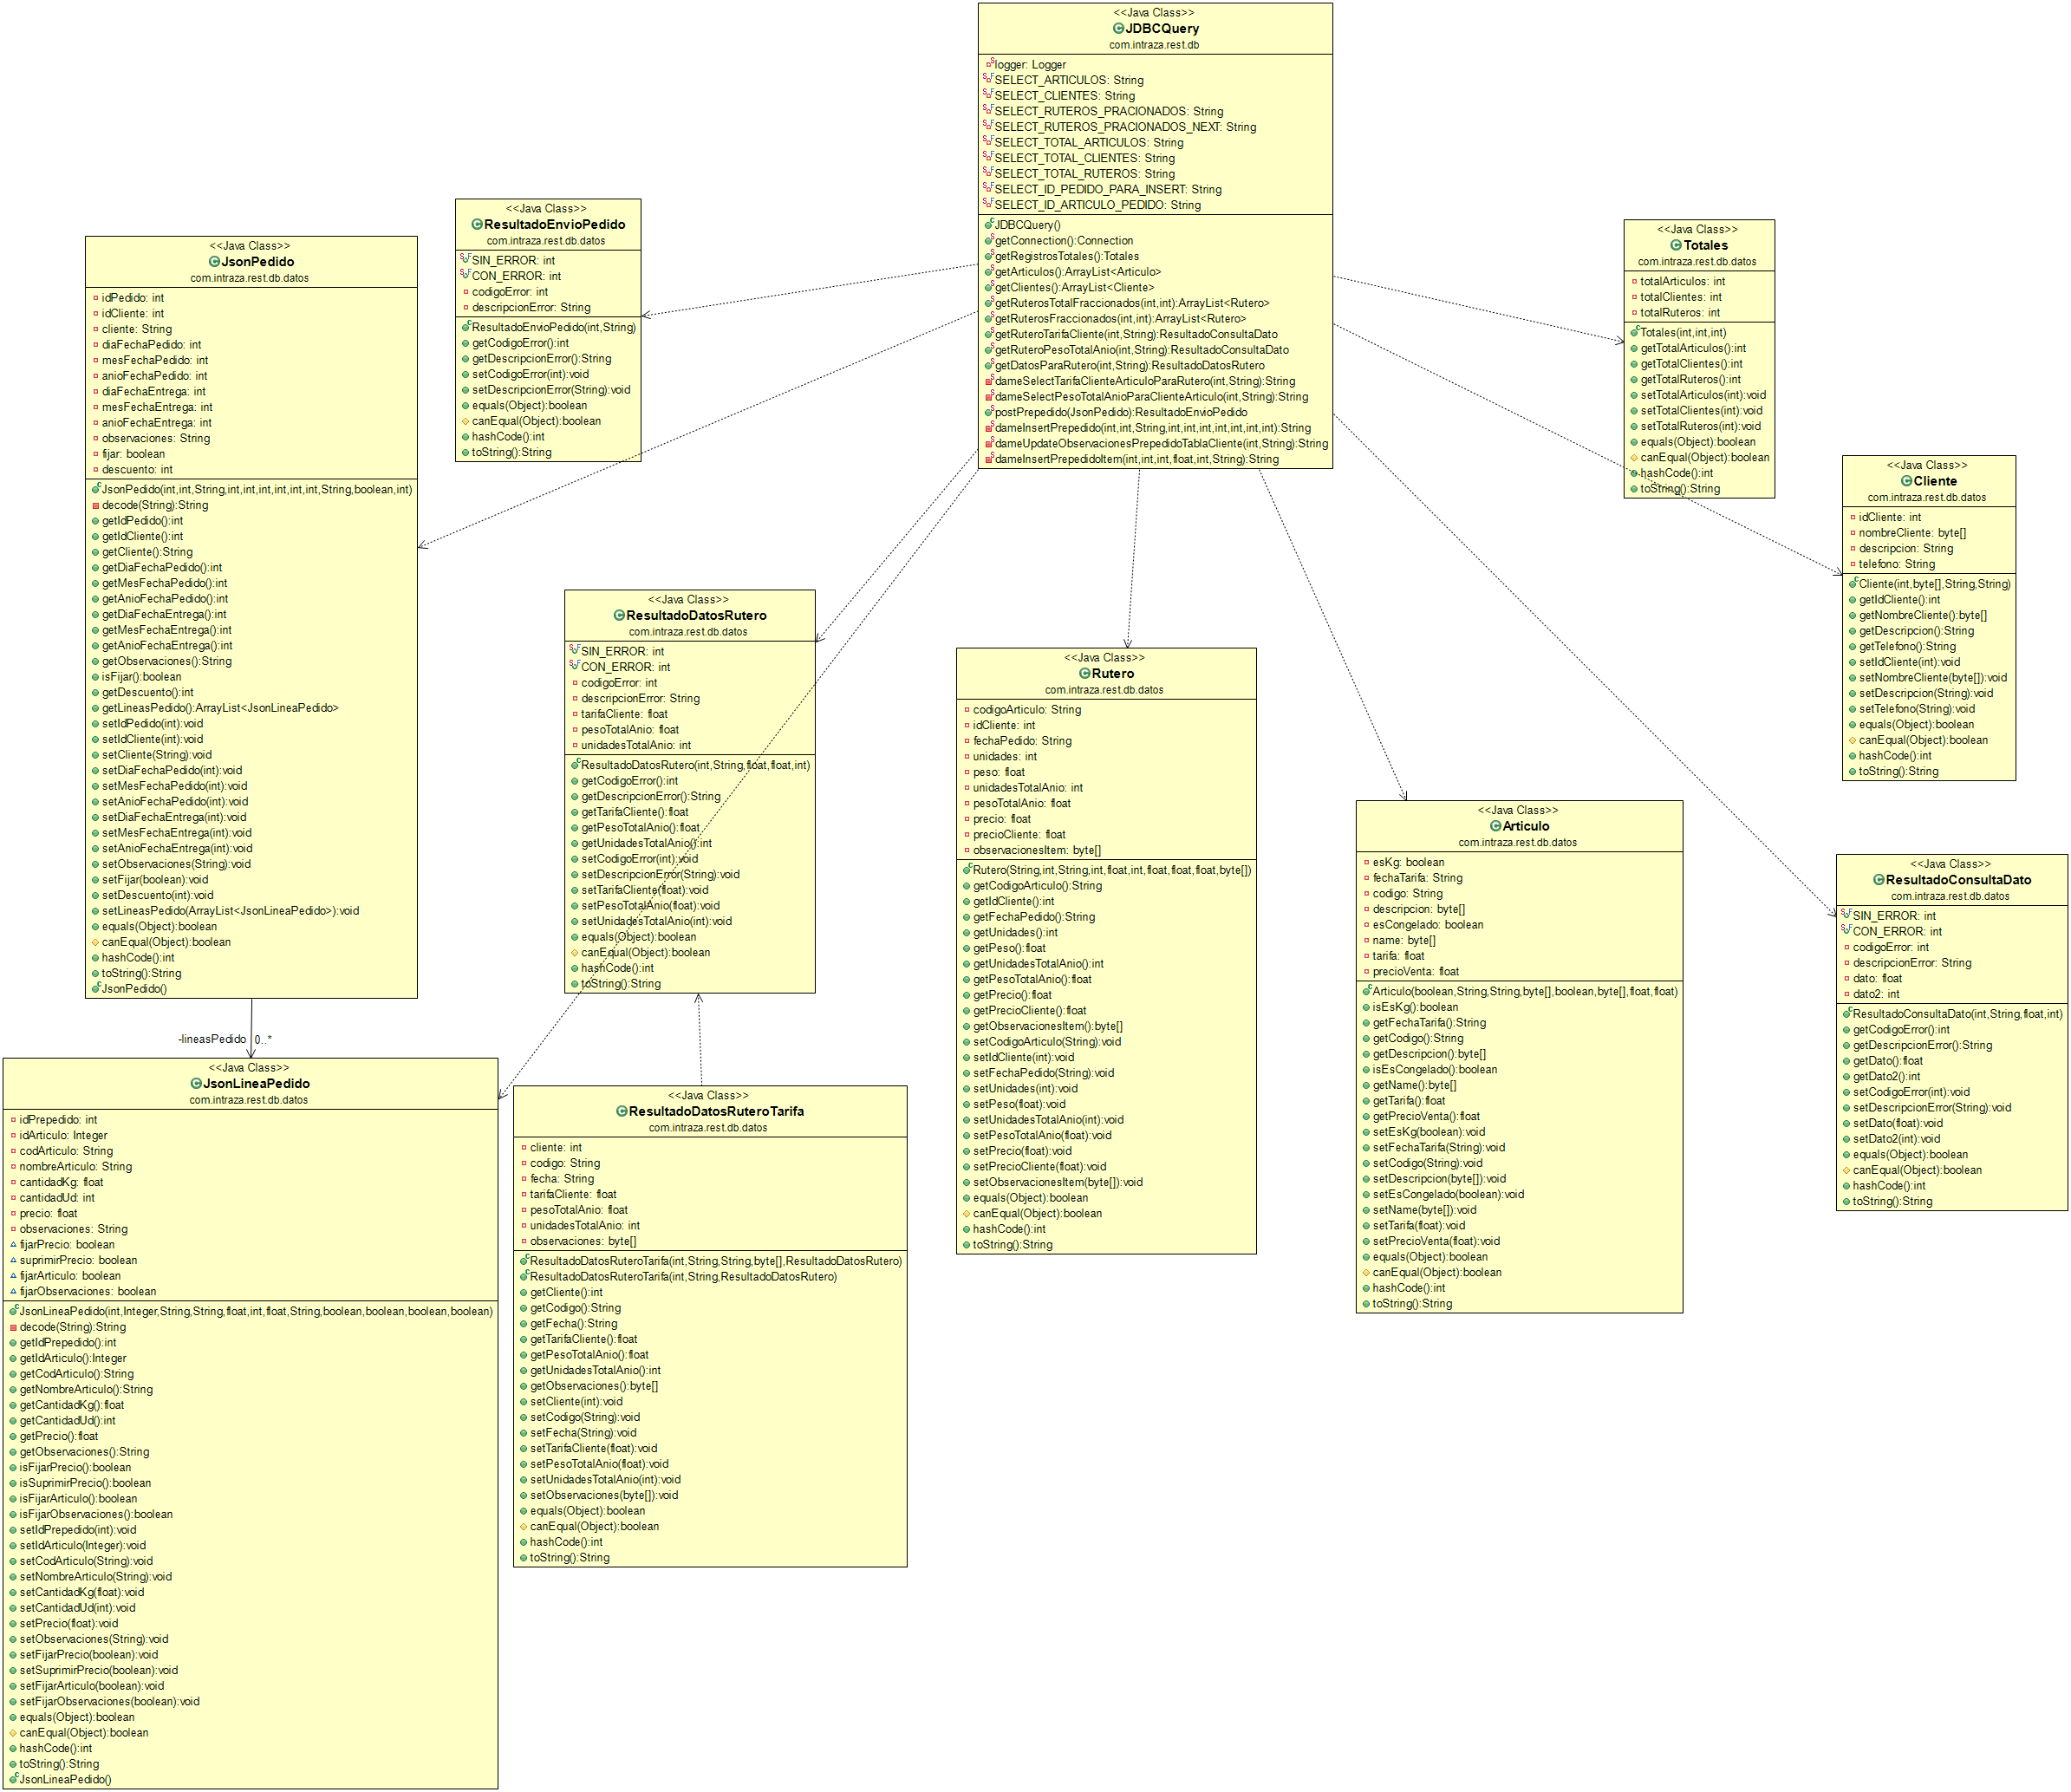
\includegraphics[width=0.9\linewidth,angle=270]{figuras/dia-web-ser-dos}}
	\caption{Relaciones JSON}
	\label{fig:dia-web-ser-dos}
\end{figure}

\pagebreak

\section{Aplicación Android}

\subsection{Descripción general}

Para el desarrollo de la aplicación Android, se ha optado por un programa nativo, usando la herramienta de desarrollo Android studio. Se ha decidido hacerla retro-compatible hasta versión 5, asegurándonos un 80\% de compatibilidad con los terminales del mercado. Como su estructura tópica ya ha sido comentada en capitulo de fundamentos, no vamos a repetir en esta sección lo ya comentado.

\begin{figure}[H]
	\centering
	
\includegraphics[width=0.7\linewidth]{figuras/app}
	\caption{Aplicaciones Android} 
	\label{fig:app}
\end{figure}

La aplicación es un interface de usuario para la gestión de pedidos mientras se encuentra desplazado, pudiendo disponer de datos de gestión de los mismos aunque no pueda establecer comunicación con el servidor. Para ello ademas de las pantallas de operación, dispondrá de una pequeña base de datos (\textbf{SQLlite}) para almacenar los datos de operación.

\subsection{Metodología empleada}

Así como el servicio disponía de \textbf{MAVEN} \textsuperscript{\textit{[\ref{glo:maven}]}} como su constructor de proyectos, en Android studio tendremos \textbf{GRADLE} \textsuperscript{\textit{[\ref{glo:gradle}]}}.

Ademas del SDK de Android dispondremos de las siguientes librerías para poder gestionar todas las necesidades operativas de la aplicación.

\begin{itemize}	
	\item \textbf{Jackson-core: } librería para la gestión de objetos JSON. 
	\item \textbf{Jackson-databind: }  librería para la gestión de objetos JSON. 
	\item \textbf{Lombok: } librería anteriormente comentada. 
	\item \textbf{Androidannotations: } librería anteriormente comentada. 
\end{itemize}

\subsection{Diseño e implementación}
Una vez tenemos la estructura de la aplicación definida, dividiremos la estructura en una actividad principal y 4 actividades secundarias para la gestión de las secciones correspondientes y por último un conjunto de clases \textit{\textbf{Dialog}} para la gestión de ventanas emergentes durante la ejecución

El almacenamiento de datos internos se realiza a través de una base de datos en SQLlite y se definen las siguientes tablas:


\begin{itemize}	
	\item TablaObservacion.
	\item TablaRutero.
	\item TablaPrepedidoItem.
	\item TablaPrepedido.
	\item TablaCliente.
	\item TablaConfiguracion.
\end{itemize}	

Para la gestión de la internacionalización\textit{(I18N)} se definen 4 archivos con los idiomas correspondientes: Castellano, Catalán, Francés, Ingles. 

Se realiza el diseño gráfico de botones, backgrounds, etc, por medio del programa Gimp, y se generan drawables para los efectos visuales del pulsado de botones.

En el ejemplo siguiente mostramos parte del código fuente correspondiente a la actividad principal de la aplicación, se puede comprobar que con las anotaciones realizadas manejamos recursos,eventos,etc, transformando la clase a un formato mas amigable.

\pagebreak

\begin{lstlisting}[style=JAVA]

@EActivity(layout.main)
public class InTrazaActivity extends Activity {
	.......	

	@AfterViews
	void init() {
		config = Configuracion.getInstance();
		config.preparaPropiedades(this);
	}	
	.......	
	
	@OnActivityResult(DIALOGO_PIDE_DATOS_NUEVO_PEDIDO)
	void onResultUno(final int resultCode, final Intent data) {
		if (Activity.RESULT_OK == resultCode) {
			final DatosPedido datosPedido = data.getParcelableExtra("DATOS_PEDIDO");
			pantallaRutero(datosPedido);
		}
		habilitaClickEnActivity(true);
	}
	.......		
}
\end{lstlisting}

Aquí vemos si lo hubiésemos escrito en el formato original java.\\


\begin{lstlisting}[style=JAVA]

public final class InTrazaActivity extends InTrazaActivity implements HasViews, OnViewChangedListener {

	private final OnViewChangedNotifier onViewChangedNotifier_ = new OnViewChangedNotifier();

	final static String DATOS_PEDIDO_EXTRA = "DATOS_PEDIDO";

	@Override
	public void onCreate(Bundle savedInstanceState) {
		OnViewChangedNotifier previousNotifier = OnViewChangedNotifier.replaceNotifier(onViewChangedNotifier);
		init(savedInstanceState);
		super.onCreate(savedInstanceState);
		OnViewChangedNotifier.replaceNotifier(previousNotifier);
		setContentView(R.layout.main);
	}

	@Override
	public<T extends View> T internalFindViewById(int id) {
		return ((T) this.findViewById(id));
	}

	private void init_(Bundle savedInstanceState) {
		Resources resources_ = this.getResources();
		..........
		OnViewChangedNotifier.registerOnViewChangedListener(this);
		..........
		injectExtras();
	}
		..........
}
\end{lstlisting}


\pagebreak

\subsection{Diagramas}
A continuación mostramos los diferentes esquemas, tanto de la base de datos como de las clases de la aplicación Android.

\begin{figure}[H]
	\centering
	\fcolorbox{black}{white}{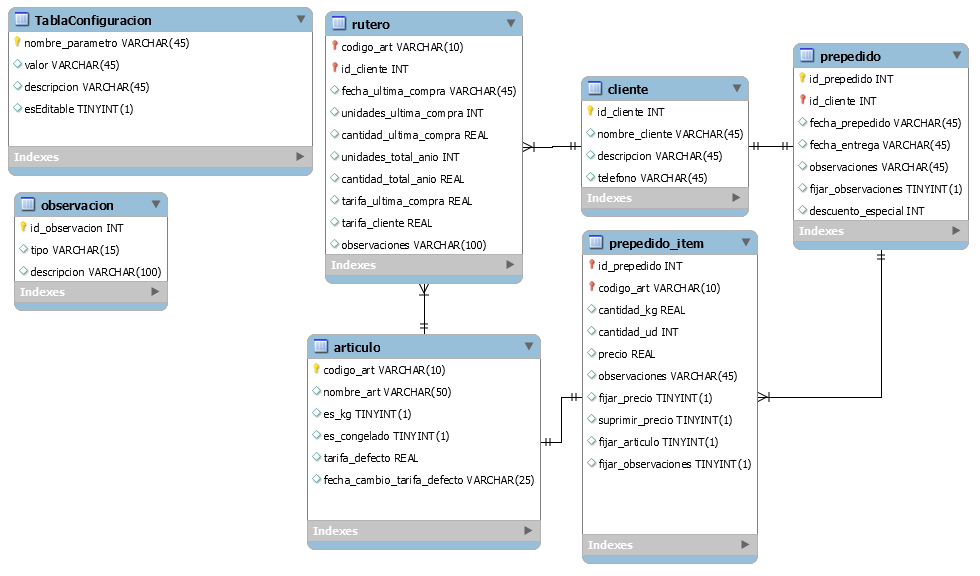
\includegraphics[width=0.6\linewidth]{figuras/eSQLlite}}
	\caption{Esquema de la base de datos SQLlite}
	\label{fig:eSQLlite}
\end{figure}

\begin{figure}[H]
	\centering
	\fcolorbox{black}{white}{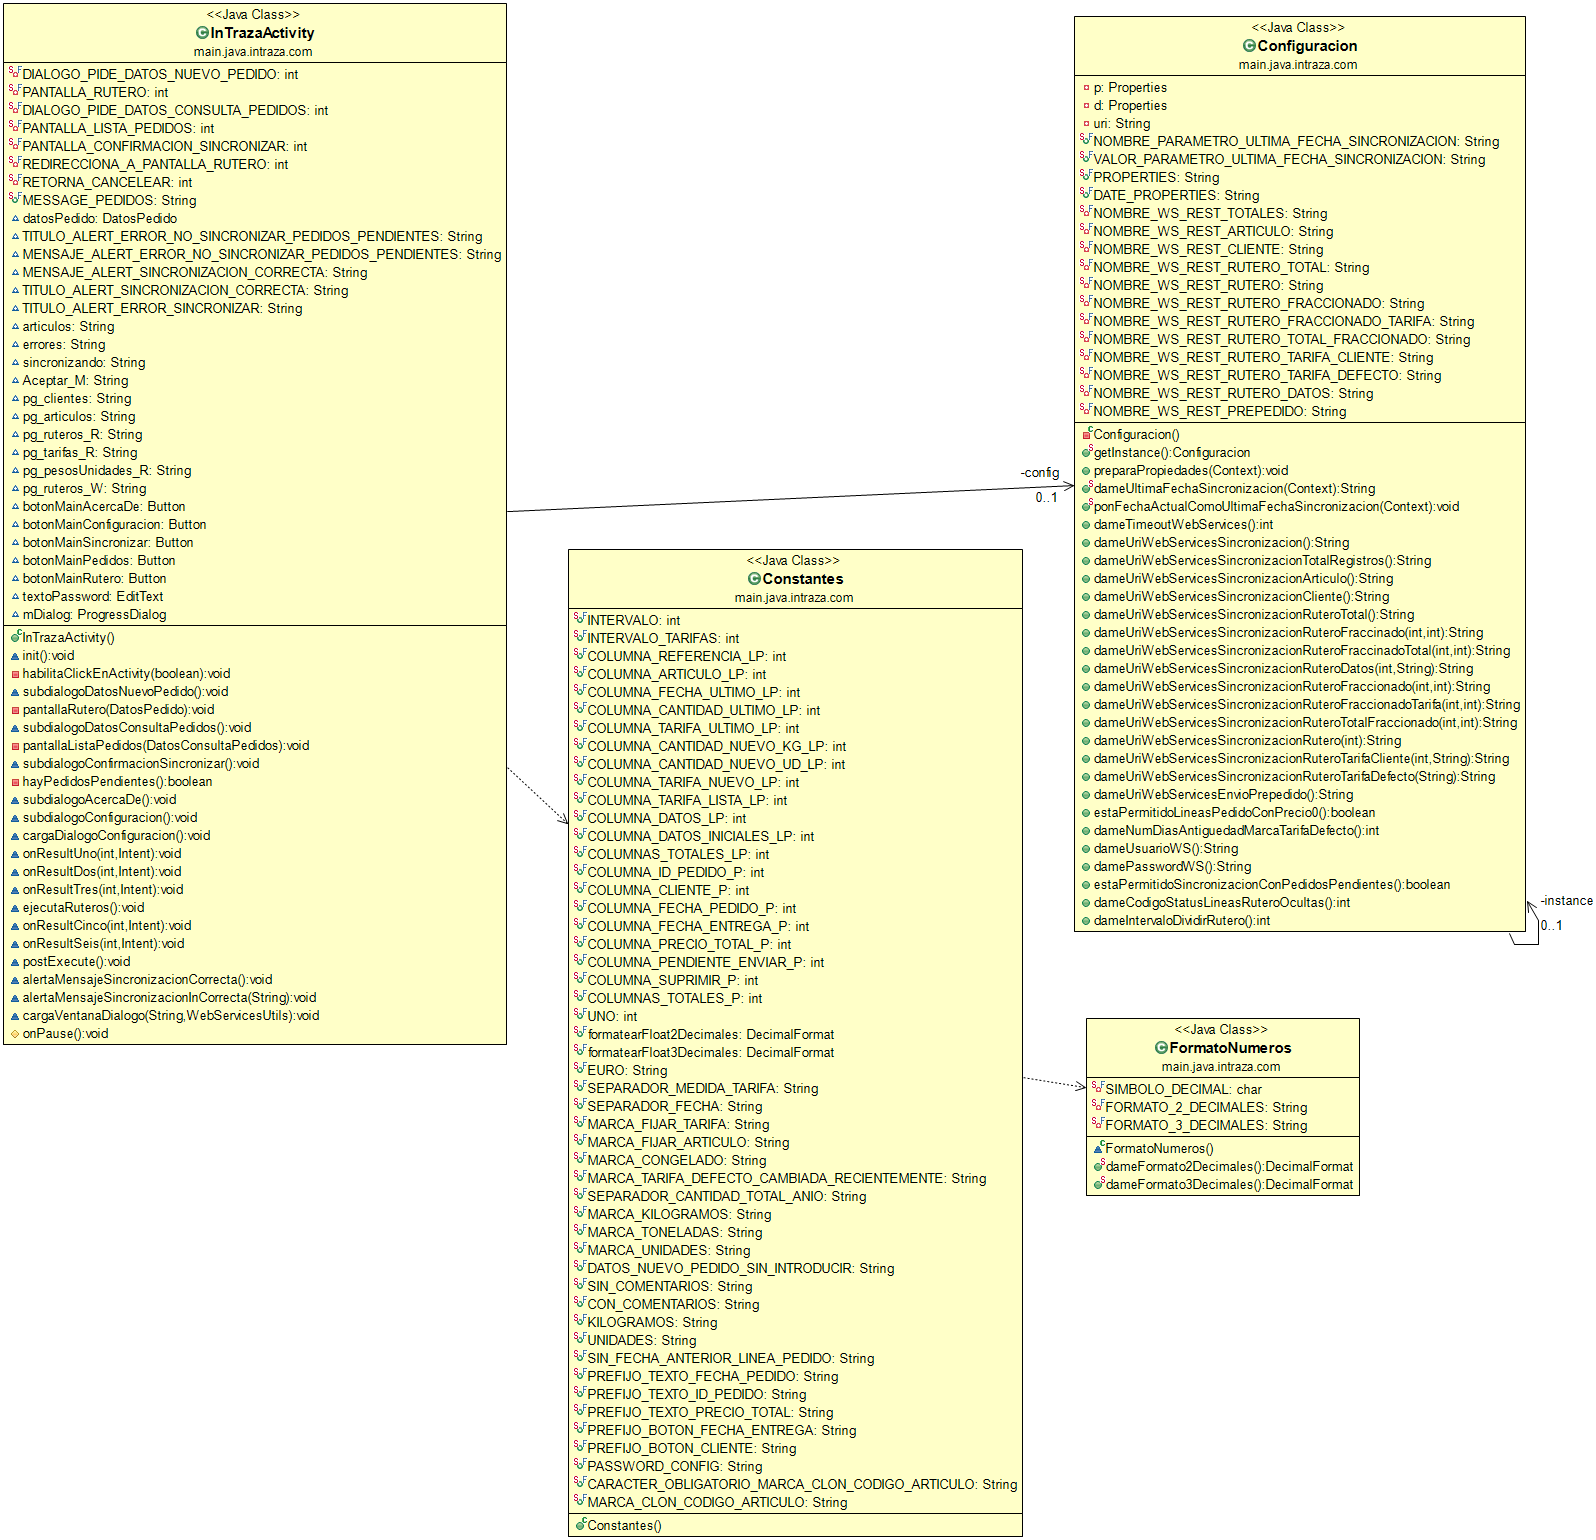
\includegraphics[width=0.6\linewidth]{figuras/and-general}}
	\caption{Esquema principal del proyecto Android} 
	\label{fig:and-general}
\end{figure}

\begin{figure}[H]
	\centering
	\fcolorbox{black}{white}{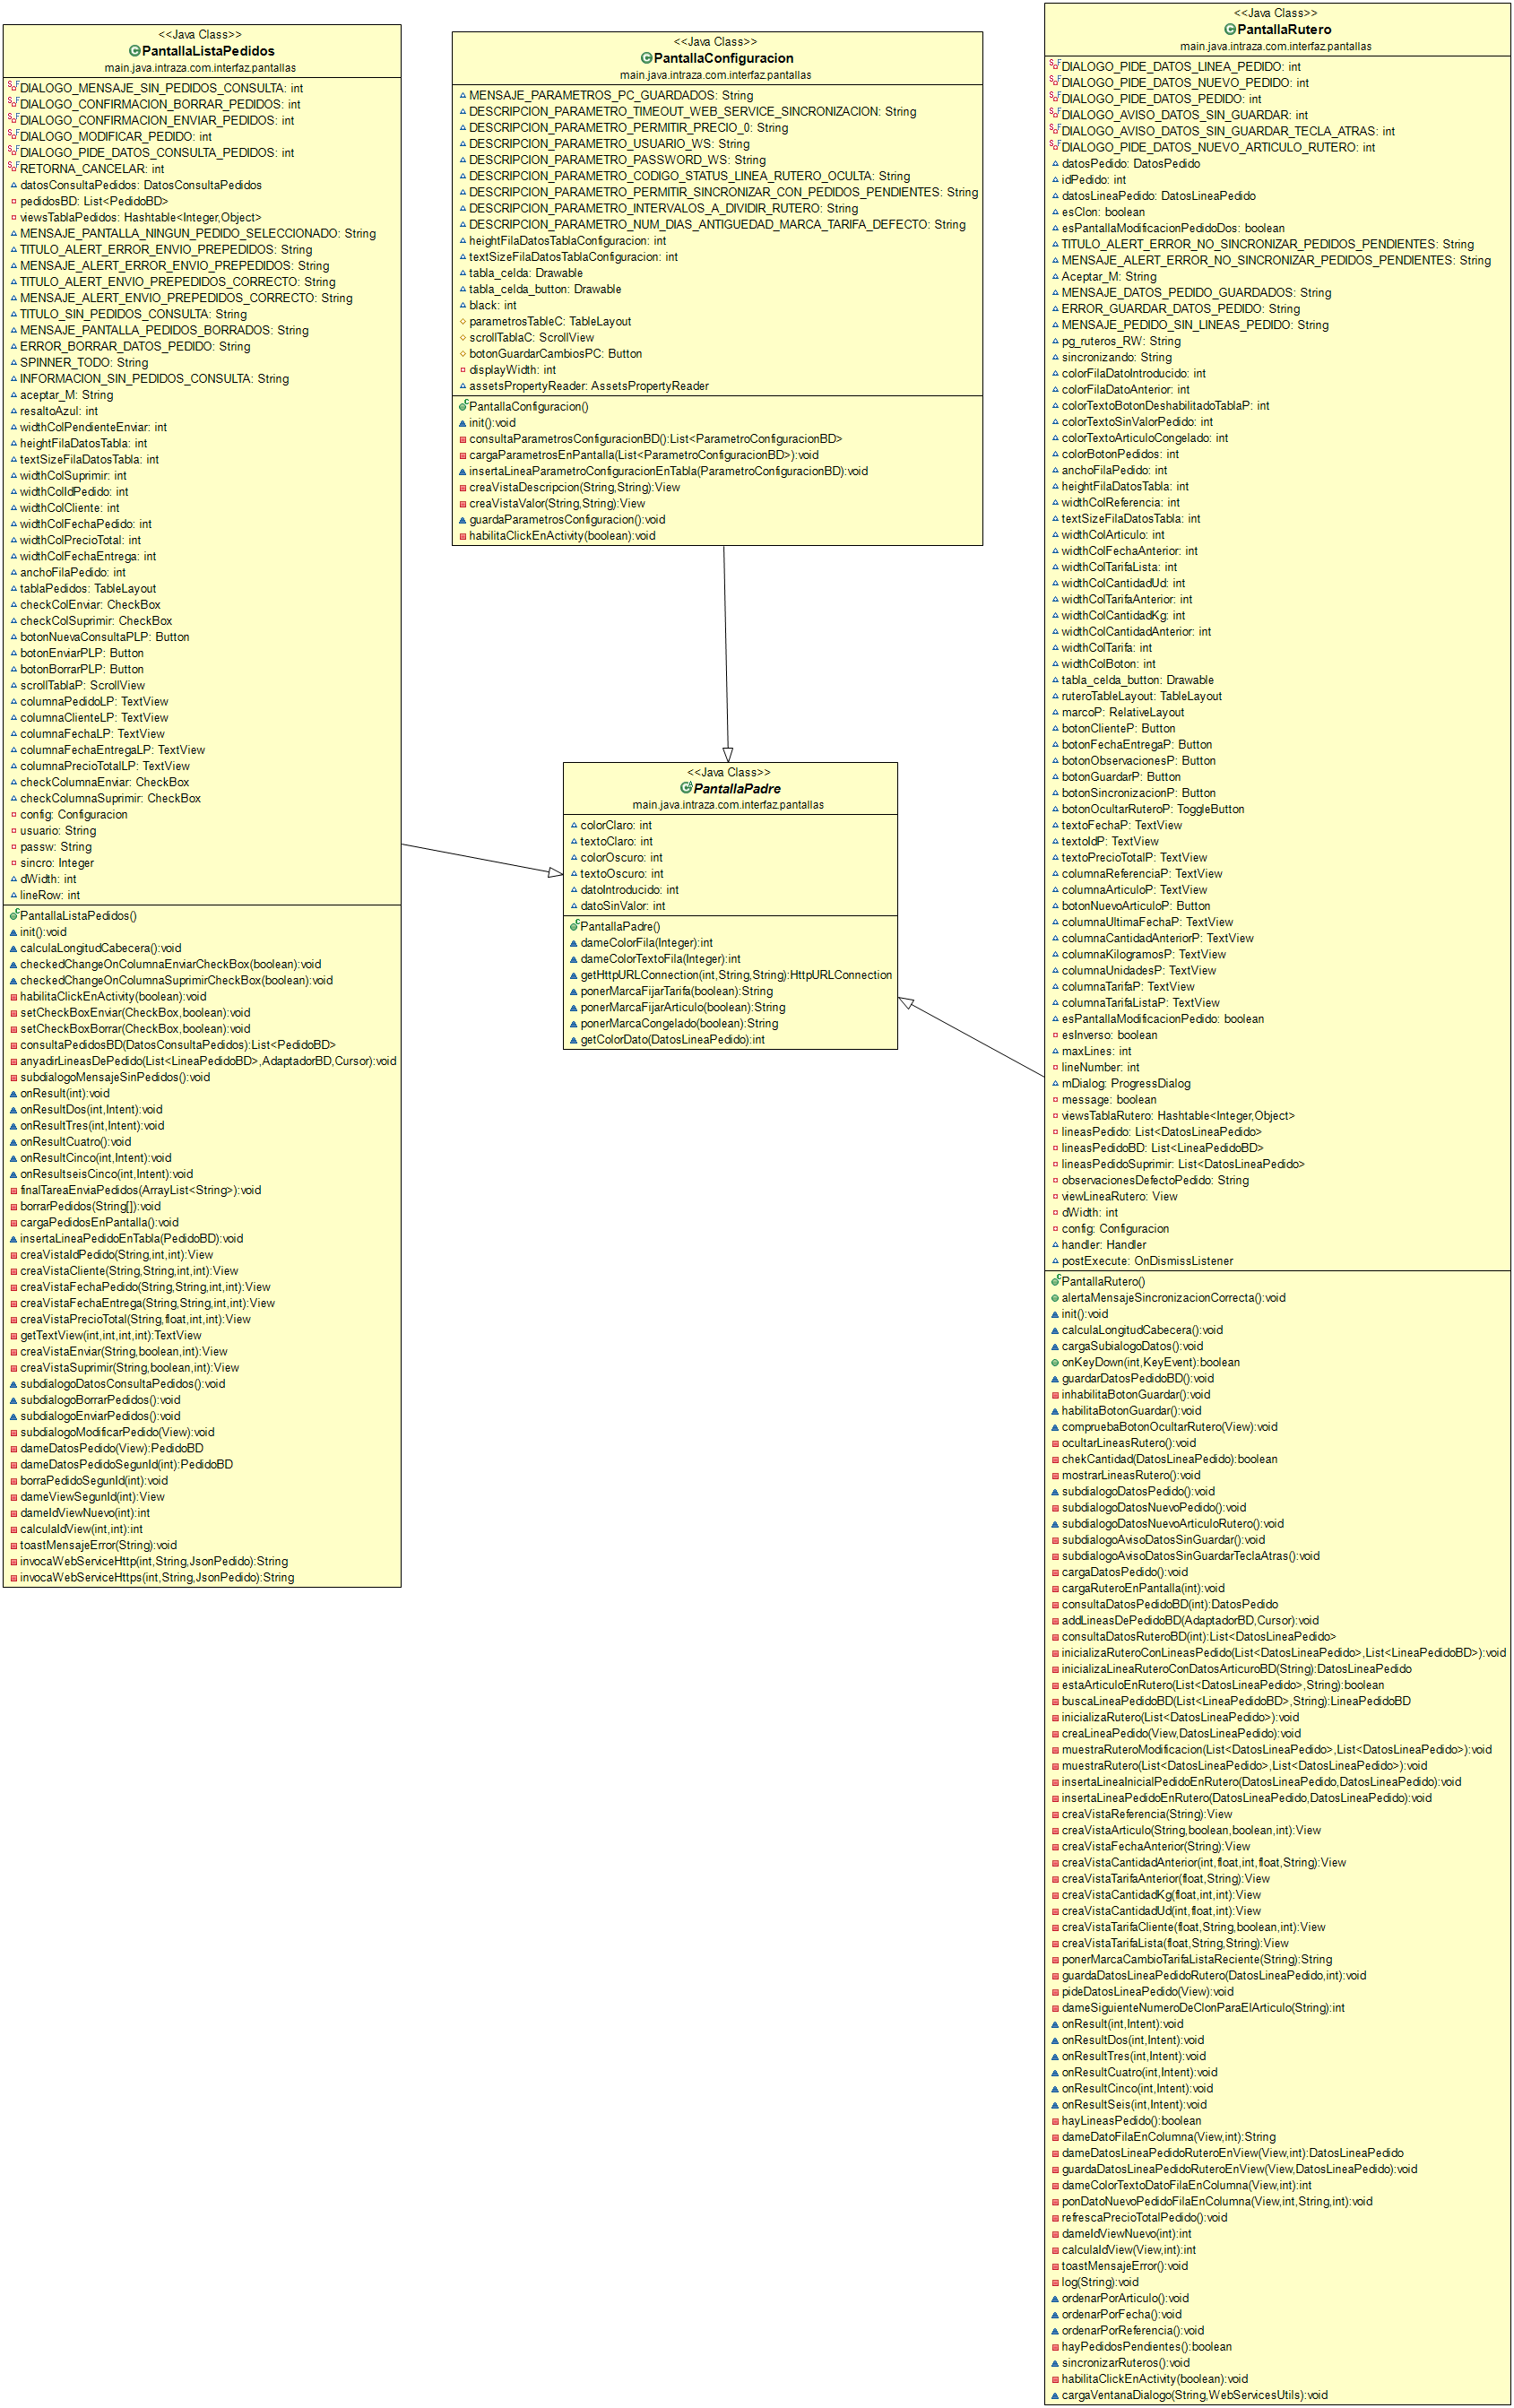
\includegraphics[width=0.8\linewidth]{figuras/and-pantallas}}
	\caption{Relaciones de datos}
	\label{fig:and-pantallas}
\end{figure}

\begin{figure}[H]
	\centering
	\fcolorbox{black}{white}{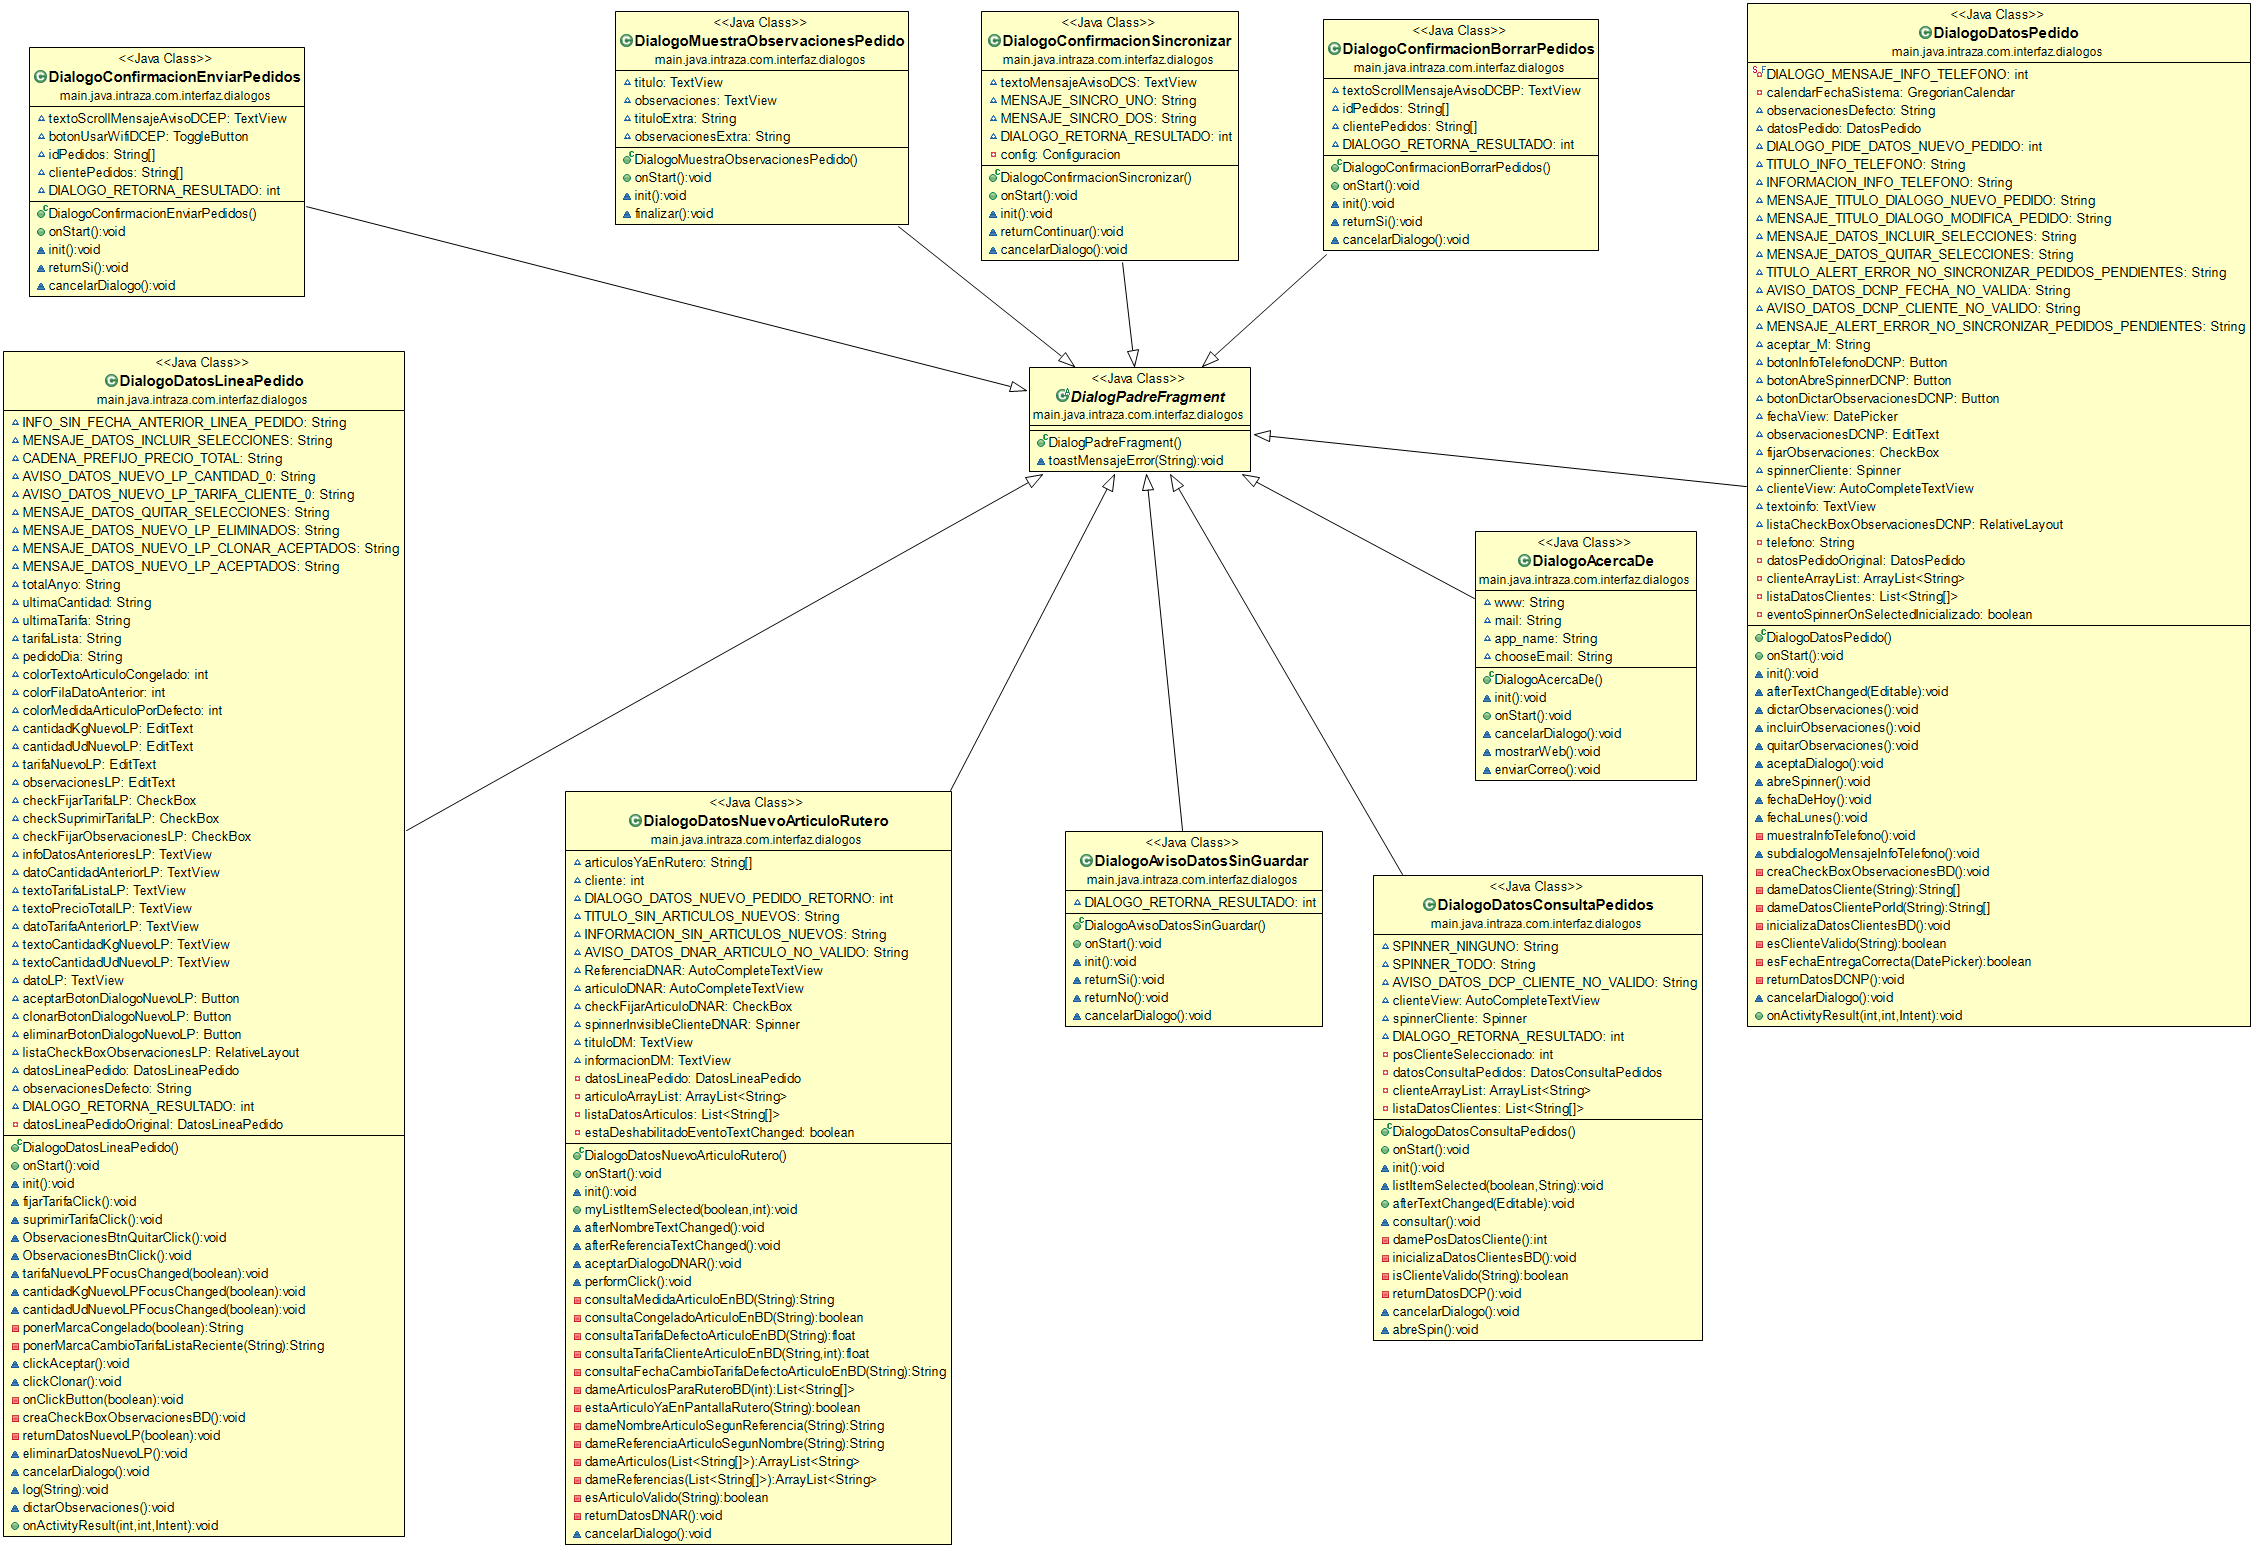
\includegraphics[width=0.7\linewidth]{figuras/and-pantallas-d}}
	\caption{Relaciones de datos}
	\label{fig:and-pantallas-d}
\end{figure}

\begin{figure}[H]
	\centering
	\fcolorbox{black}{white}{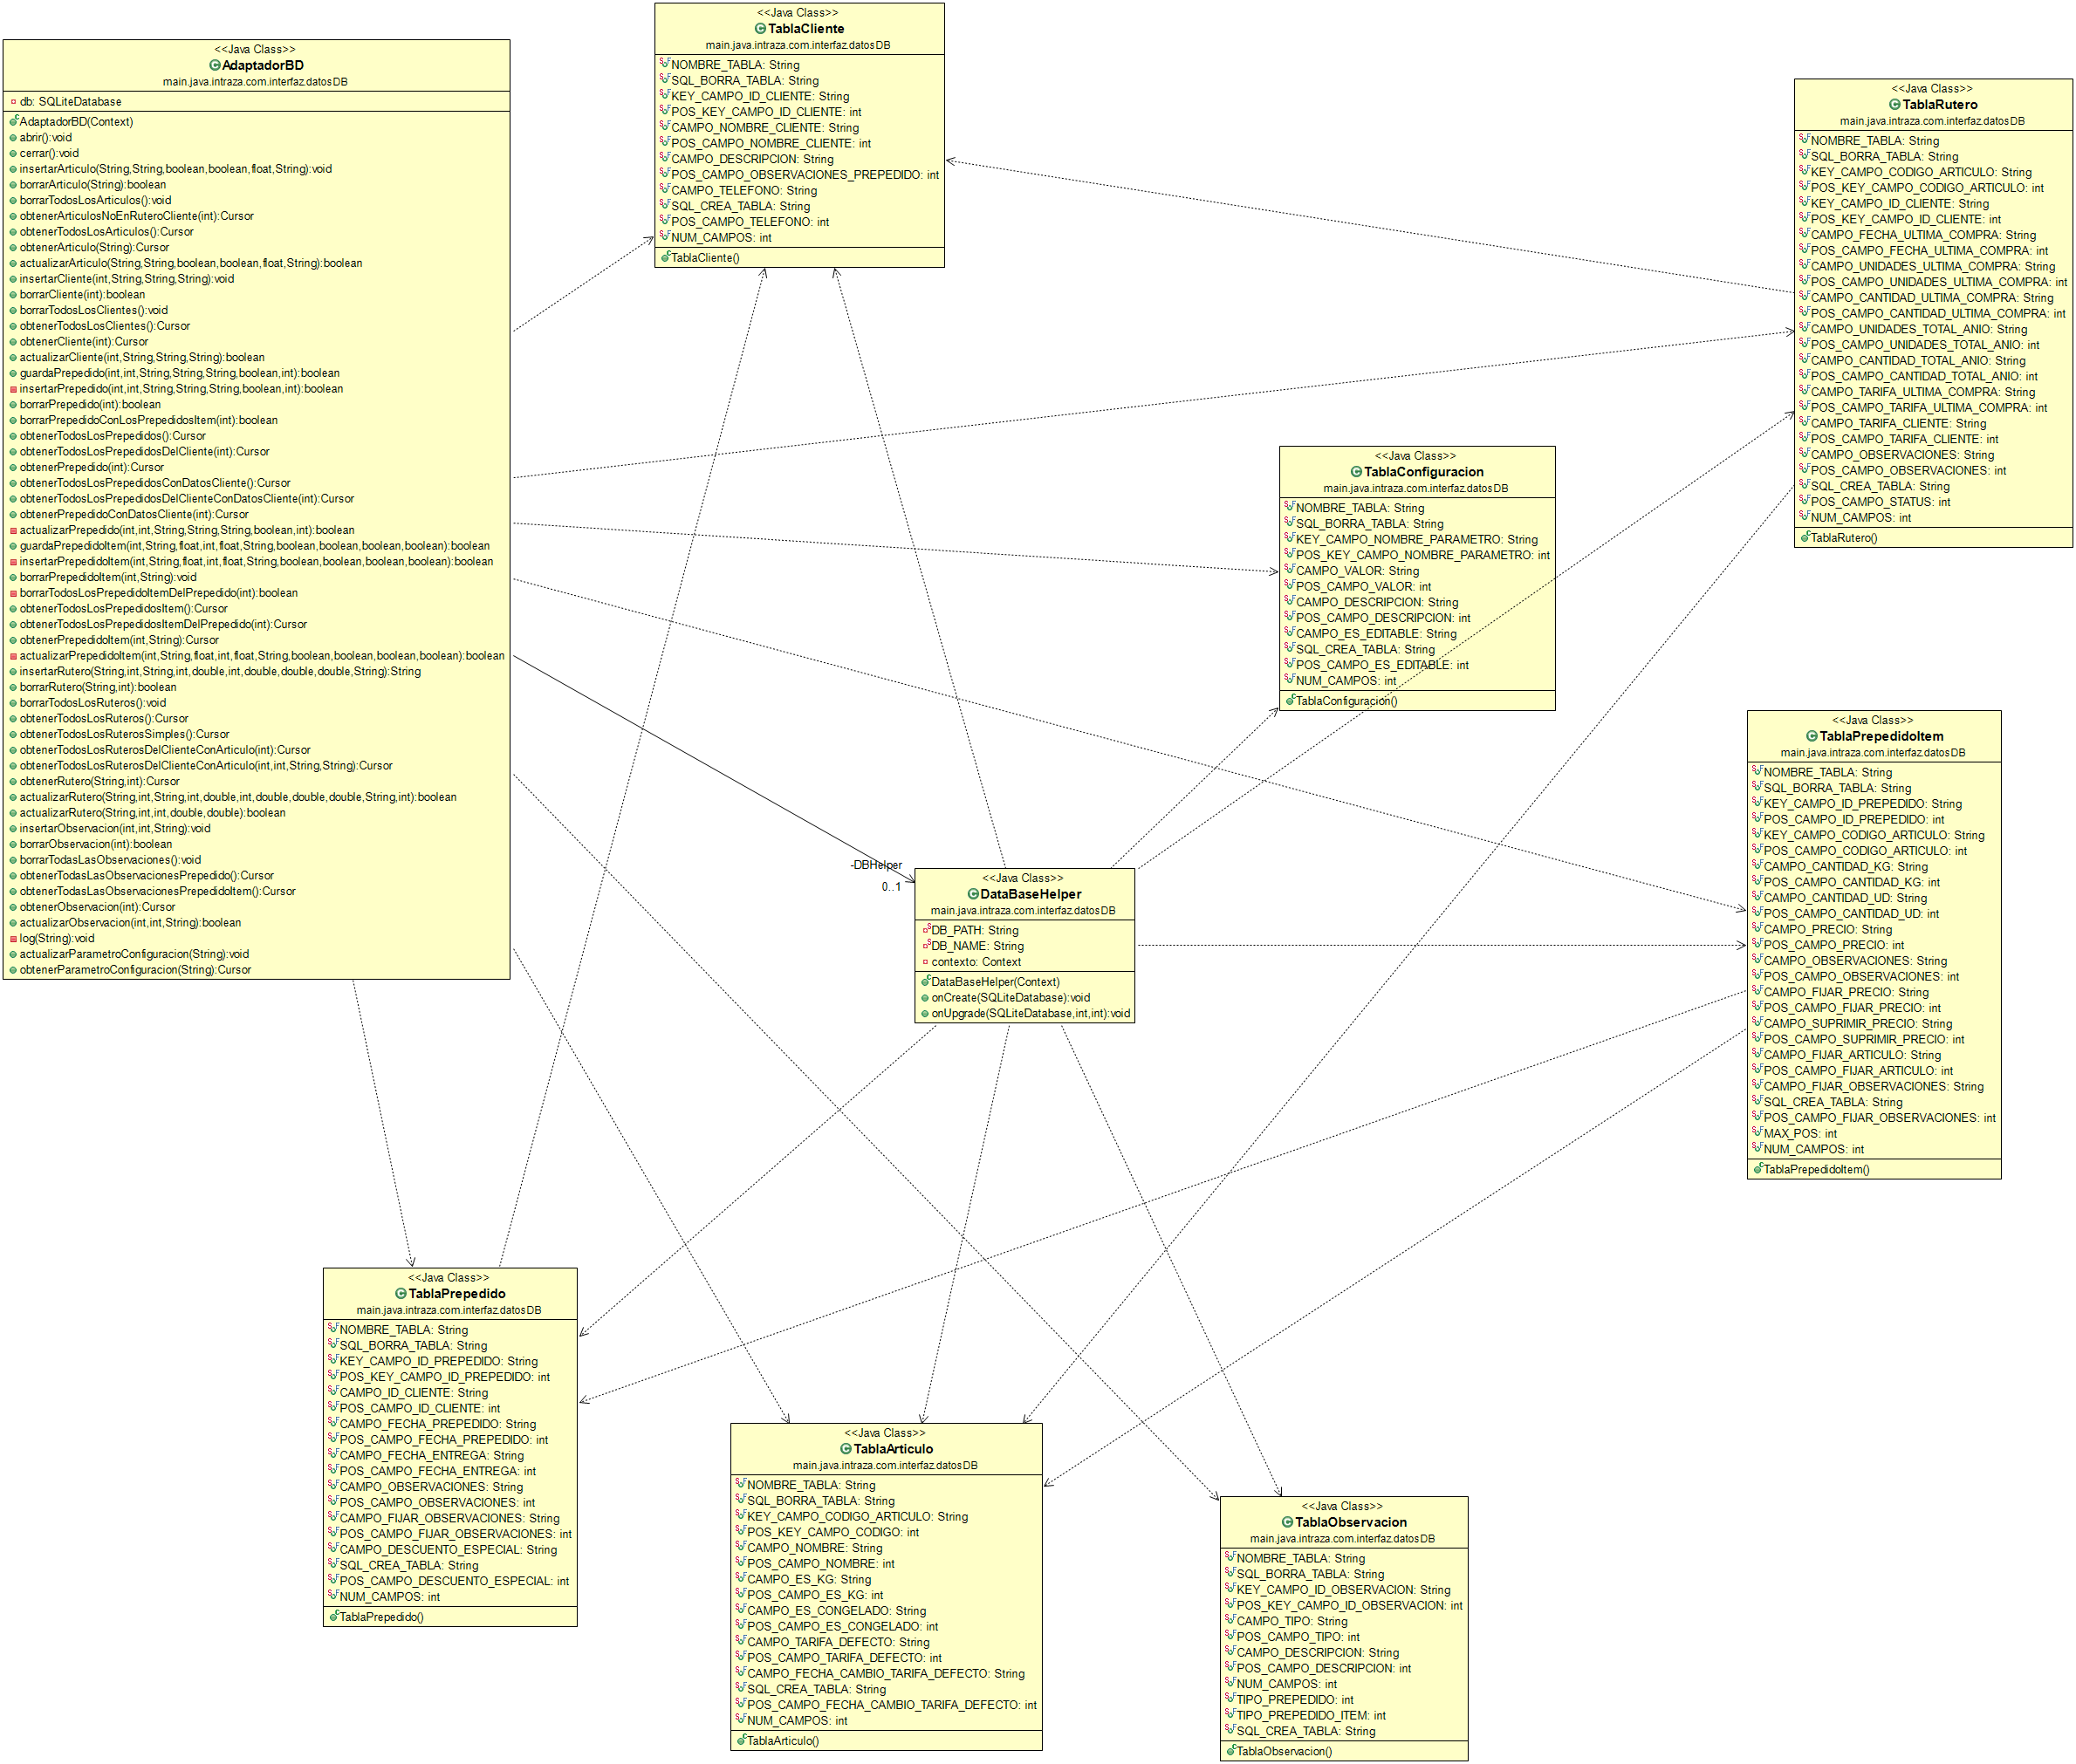
\includegraphics[width=0.7\linewidth]{figuras/and-Db}}
		\caption{Relaciones JSON}
		\label{fig:and-Db}
	\end{figure}

\subsection{Pruebas}

Debido a la imposibilidad de realizar las simulaciones, frente a un entorno de desarrollo de la empresa cliente, por las razones ya expuestas anteriormente, se decide crear una estructura de simulación propia. 

\subsubsection{Desarrollo del ERP de simulación}

Una de las cosas a tener en cuenta, a la hora de desarrollar el ERP\textsuperscript{\textit{[\ref{glo:erp}]}} de pruebas, es que debe ser rápido en su codificación y con una complejidad suficiente para poder realizar todas las pruebas de comunicación.

Con esas premisas, se opta por realizar el aplicativo usando un Framework ligero. La elección es GRAILS\textsuperscript{\textit{[\ref{glo:gra}]}} , un Framework escrito en Groovy y compatible con los entornos JAVA.

El uso de un lenguaje dinámico, de sintaxis parecida a JAVA y su principal peculiaridad de que abarca las tres capas del desarrollo web: acceso a base de datos, capa de negocio y vista, permiten acortar los tiempos de desarrollo notablemente.

Ademas de lo anteriormente dicho, añadiendo herencias y usando reflexión nos encaminan a disponer un producto totalmente operativo en unos pocos días.

\subsubsection{Estructura Básica}

Definiremos una estructura básica compuesta por :
\begin{itemize}	
	\item \textbf{Clases dominio: } Serán el equivalente a las tablas en la base de datos. 
	\item \textbf{Controladores: } Serán los encargados de trazar los flujos de operación, al navegar por las diferentes vistas. 
	\item \textbf{Servicios: } Serán los encargados de proporcionar todas las operaciones de comunicación con agentes externos, filtros y demás código necesario. 
	\item \textbf{Vistas: } Serán las que proporciones las pantallas de la vista del modelo MVC. 
	\item \textbf{TagLibs: } Serán librerías de utilidades para agilizar o simplificar procesos mas complejos en las vistas. 
\end{itemize}

Aquí tenemos un ejemplo de código perteneciente a la clase controlador principal. Corresponde a una acción de listado genérica.
\pagebreak

\begin{lstlisting}[style=JAVA]
private doList() {
	//offset
	doBefore()
	def entidad = clazz
	
	if (entidad) {
		instanceTotal = entidad?.count()
		params.max = Math.min(params.max ? params.int('max') : 10, 100)

	if (params.offset) 
		offset = params.offset
	else if (instanceTotal > offset) 
		params.offset = offset
	
	if (params.sort || !sort)
		instanceList = entidad.list(params)
	else
		instanceList = entidad.list(max: params?.max, offset: params?.offset, sort: sort[0], order: sort[1])
	}
	render(view: 'list', model: mapaVariables(), params: params)
}

\end{lstlisting}

Aquí un ejemplo de acciones de un controlador para el dominio Pedido. Se puede ver que la mayoría del código es procesado por una clase padre, y solo definimos particularidades si lo necesitamos. La creación de nuevas entidades se simplifica, y disponemos de un alto porcentaje de reutilización de código.

\begin{lstlisting}[style=JAVA]
package pedido
import controller.MainController

class PedidoController extends MainController {
	def pedidoService
	def index() 		{ super.doIndex() 			  }
	def list() 			{ super.doList() 			  }
	def create() 		{ super.doCreate() 			  }
	def save() 			{ super.doSave()  			  }
	def show() 			{ super.doShow()  			  }
	def edit() 			{ super.doEdit()  			  }
	def update() 		{ super.doUpdate()  		  }
	def delete() 		{ super.doDelete()    		  }
	def limpiarFiltro() { super.doLimpiarFiltro()     }
	def ajx_filtrar()	{ super.doAjx_filtrar()       }
}
\end{lstlisting}


\subsubsection{Diseño de la base de datos ERP}

Nos planteamos un diseño base de datos sencillo con las tablas básicas que debería tener el ERP. Evidentemente un ERP comercial tendrá mayor complejidad, pero este desarrollo es para realizar un entorno de pruebas. En la figura siguiente planteamos el esquema de tablas y relaciones.

\begin{figure}[H]
	\centering
	\fcolorbox{black}{white}{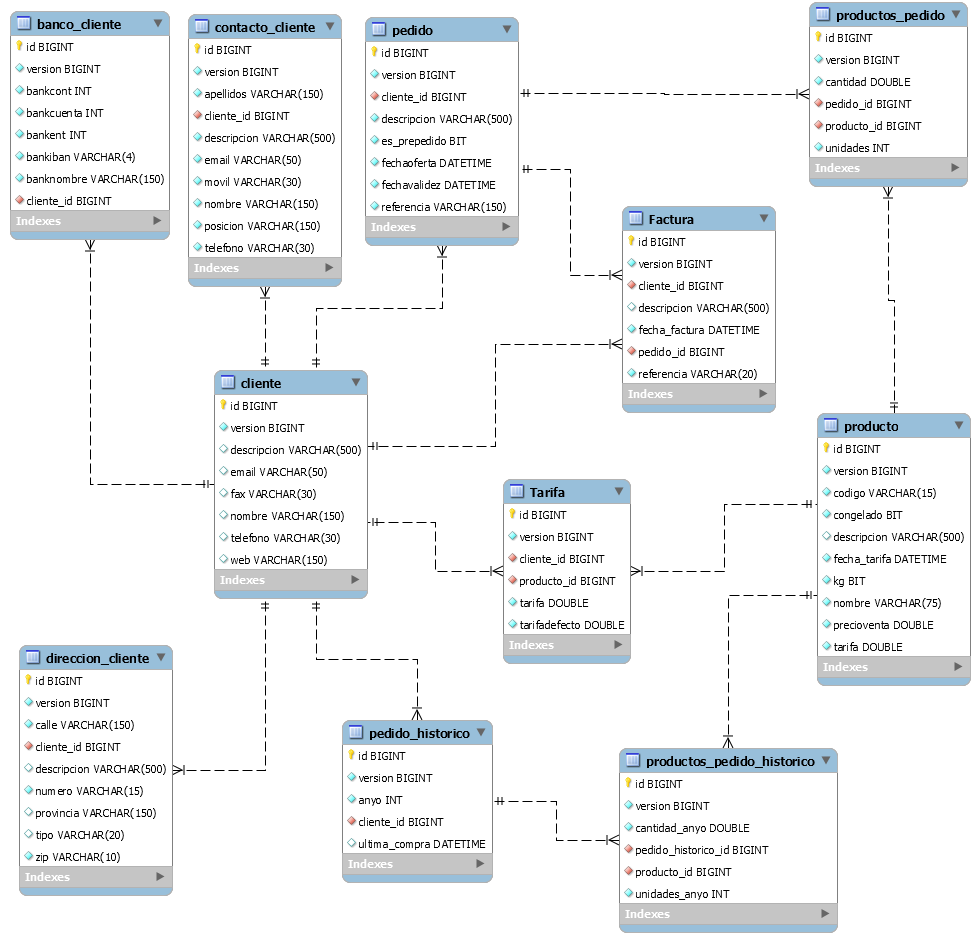
\includegraphics[width=0.7\linewidth]{figuras/grailsM}}
	\caption{Modelo de datos del ERP }
	\label{fig:pruebas-datos}
\end{figure}
